%\setchapterimage{fig_00}
\chapter*{Colle \arabic{cptColle} \\
Imagerie médicale -- \ifprof Corrigé \else Sujet \fi}

\addcontentsline{toc}{section}{Colle \arabic{cptTD} : Imagerie médicale -- \ifprof Corrigé \else Sujet \fi}

\iflivret \stepcounter{cptColle} \else
\ifprof  \stepcounter{cptColle} \else \fi
\fi
\setcounter{question}{0}

\marginnote{F. Mathurin.}




\begin{marginfigure}
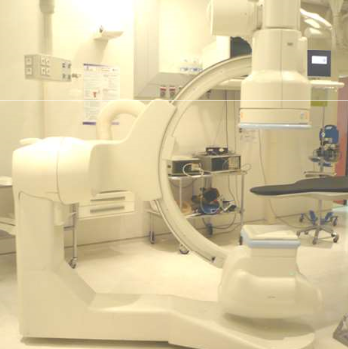
\includegraphics[width=\linewidth]{fig_02_01}
%\textit{}
\end{marginfigure}

\begin{marginfigure}
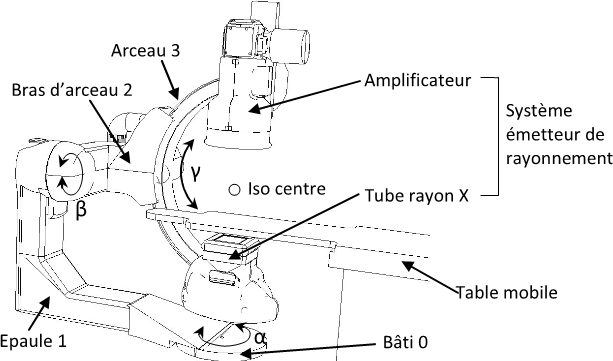
\includegraphics[width=\linewidth]{fig_02_02}
%\textit{}
\end{marginfigure}

L'étude porte sur un système permettant de réaliser des imageries médicales de vaisseaux sanguins sur un patient. Ce système, conçu par General Electric Medical System, envoie des rayons X dans le corps du patient et mesure leur rayonnement. En fonction des informations reçues, une image de synthèse en 3 dimensions est réalisée, permettant de voir les éventuels problèmes médicaux à venir. 

 Ce système est constitué des éléments suivants : le bâti 0, une épaule 1 qui peut être mis en mouvement par rapport au bâti 0, un bras d’arceau 2 qui peut s’orienter par rapport à l’épaule 1 et un arceau 3 qui se déplace par rapport à bras d’arceau 2. Le patient est situé sur une table mobile. Le réglage en hauteur du patient sur la table mobile est possible pour son confort mais n'est pas utilisé au cours d'une analyse. Seuls les degrés de liberté $\alpha$, $\beta$ et $\gamma$ sont utilisés pendant l’analyse. L'émetteur de rayons, situé sur l'arceau, focalise la vision interne du patient en un point appelé iso centre. 

\begin{marginfigure}
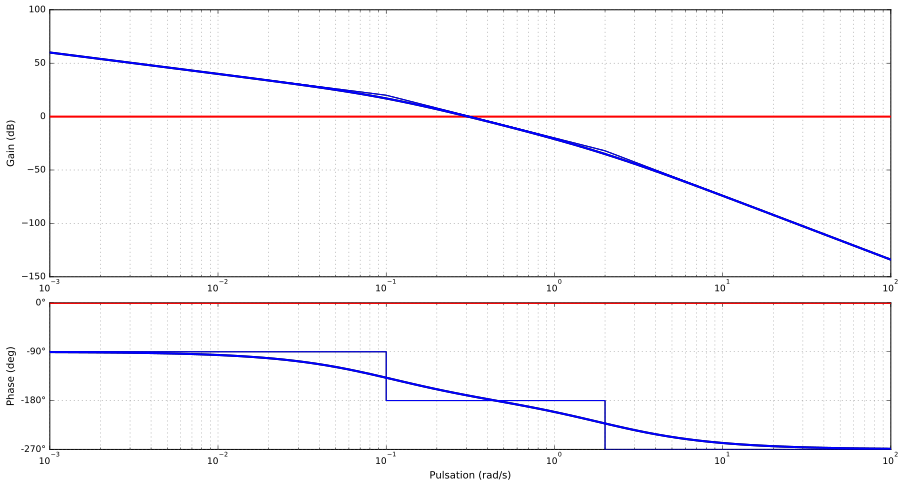
\includegraphics[width=\linewidth]{fig_03}
%\textit{}
\end{marginfigure}

Sur l’image de gauche, l’arceau 3 s’oriente par rapport au bras d’arceau 2 et sur l’image de droite le bras d’arceau 2 se déplace par rapport à l’épaule 1. On donne ci-dessous un extrait de cahier des charges fonctionnel du système de positionnement dans la phase de vie correspondant à une mesure d'imagerie : 

\begin{center}
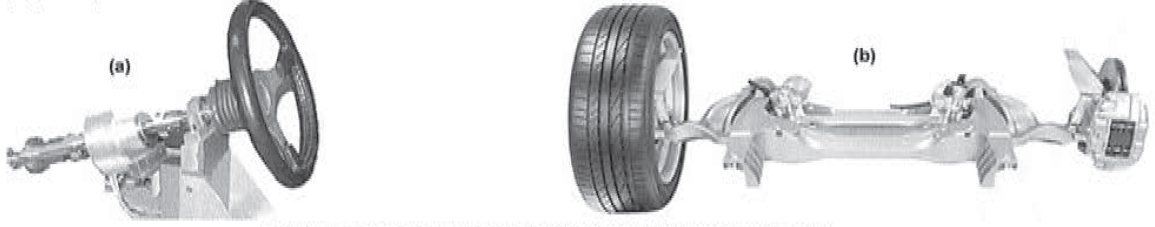
\includegraphics[width=\linewidth]{fig_07}
%\textit{}
\end{center}

%
%\question{Déterminer le nombre de mouvements élémentaires utilisés (translation ou rotation) pour orienter le faisceau de rayon. }

Conformément au cahier des charges, chaque axe élémentaire, piloté séparément, doit avoir une vitesse angulaire de $10^{\text{o}}\text{/s}$ en phase de mesure. Technologiquement, la chaine d’action de chaque axe élémentaire est constituée d’un réducteur entre le moteur et l’effecteur. Ce réducteur diminue la vitesse angulaire d'un facteur 558. 

%\question{Déterminer la vitesse angulaire de chaque moteur (en tr/min) qui permet de satisfaire le critère de vitesse angulaire du cahier des charges. }

On s’intéresse à l’axe permettant de déplacer le bras d’arceau 2 par rapport à l’épaule 1. La structure de la chaine fonctionnelle asservie de cet axe est la suivante : 
\begin{center}
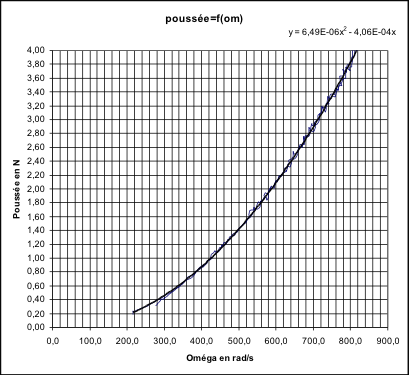
\includegraphics[width=\linewidth]{fig_04}
%\textit{}
\end{center}


Les différents éléments de cette chaîne fonctionnelle sont les suivants :
\begin{itemize}
\item l'amplificateur est un gain pur : $K_a$;
\item le réducteur est un gain pur $K_r$ (sans dimension);
\item le capteur est un gain pur : $K_c$;
\item le moteur est un système d'ordre 1, de constante de temps $T_m$ et de gain $K_m$. On note la fonction de transfert du moteur $H_m (p)$. 
\end{itemize}

\question{Déterminer la valeur numérique du bloc du réducteur $K_r$. }


\question{Déterminer la fonction de transfert en chaîne directe $\text{FTCD}(p)$, la fonction de transfert en boucle ouvert $\text{FTBO}(p)$ et la fonction de transfert en boucle fermée $\text{FTBF}(p)$ de cet asservissement. Exprimer les résultats en fonction de $K_a$, $K_m$, $K_r$, $K_c$ et $T_m$. }


\question{Montrer que la fonction de transfert en boucle fermée de ce système peut s'écrire sous la forme d'un deuxième ordre $\dfrac{K}{1+\dfrac{2z}{\omega_0}p+\dfrac{p^2}{\omega_0^2}}$. Donner l’expression littérale de $K$, $z$ et $\omega_0$ en fonction de $K_a$, $K_m$, $K_r$, $K_c$ et $T_m$ . }


%\question{Déterminer la réponse du moteur $\omega_m (t)$ à une entrée en échelon de tension $u_m (t)$ de la forme $u_m (t)  = U_0 u(t)$ ($U_0$ valant \SI{10}{V}). Exprimer le résultat en fonction de $U_0$ , $K_m$ et $T_m$. }


\question{La réponse du système à cette entrée en échelon de tension $u_m (t) =10u(t)$ a été mesurée en sortie du réducteur. On donne ci-contre la courbe obtenue. Déterminer les valeurs numériques expérimentales de $K_m$ et $T_m$ à partir de la courbe.}

\vspace{.5cm}

Avec les valeurs numériques des coefficients des différents gains, on peut déterminer la valeur numérique de a fonction de transfert en boucle ouverte : $\text{FTBO}(p)=\dfrac{10}{p\left(1+\dfrac{1}{30}p\right)}$.

\question{Tracer les diagrammes de Bode asymptotiques de la fonction de transfert en boucle ouverte sur le diagramme vierge en bleu. }


\question{Calculer le gain et la phase exacte pour $\omega = \SI{30}{rad/s}$.}


\begin{marginfigure}
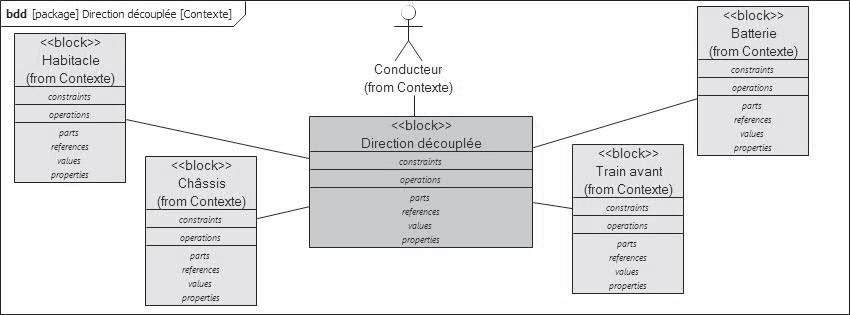
\includegraphics[width=\linewidth]{fig_05}
\end{marginfigure}

\question{On donne les tracés réels des courbes de gain et de phase de la FTBO. Déterminer la pulsation qui annule le gain puis déterminer la marge de phase du système M$\varphi$. Conclure quant à la capacité du système à satisfaire le critère de marge de phase du cahier des charges. }

\begin{center}
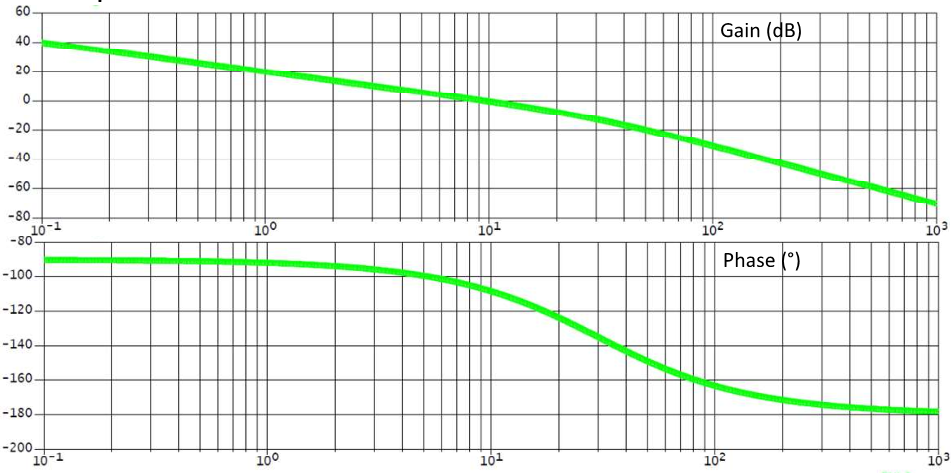
\includegraphics[width=\linewidth]{fig_06}
\end{center}



\begin{center}
\begin{tikzpicture}[xscale=16/10]
\tikzset{
semilog lines/.style={thin, bleuxp}, 
semilog lines 2/.style={semilog lines,bleuxpc},
semilog half lines/.style={semilog lines 2,dotted },
semilog label x/.style={semilog lines,below,font=\tiny,black},
semilog label y/.style={semilog lines,right,font=\tiny,black}
}
\begin{scope}[yscale=6/150]
\OrdBode{10}
\semilog{-2}{4}{-60}{20}

%\BodeGraph[orangexp,samples=150,ultra thick]{-3:3}{-\SOAmp{1}{.1}{1}+\IntAmp{0.01}+\POAmp{1}{0.01}}

%\BodeAmp[orangexp,thin,samples=150]{-2:2}{\SOAmpAsymp{10}{0.2}{.9}}
%s\BodeAmp[orangexp,ultra thick,samples=150]{-2:2}{\SOAmp{10}{0.2}{.9}}
%\draw (-1.5,28) node {\footnotesize $20\log K$};
%\draw (1.1,10) node {\footnotesize $-$40 dB/d\'ecade};
%\draw [dashed,ultra thick,bleuxp] (-.08,-60) -- (-.08,25);
%\draw (-.08,-60)  node {\Huge $\cdot$} node [above right]{\footnotesize $\omega_0$};
\end{scope}
\begin{scope}[yshift=-4cm,yscale=1/90]
\UniteDegre
\OrdBode{45}
\semilog{-2}{4}{-180}{90}
%\BodeArg[orangexp,samples=150,ultra thick]{-3:3}{-\SOArg{1}{.1}{1}+\IntArg{0.01}+\POArg{1}{0.01}}
%\BodeArg[orangexp,samples=100,thin]{-2:2}{\SOArg{10}{0.2}{.9}}
%\BodeArg[orangexp,ultra thick]{-2:2}{\SOArg{10}{0.2}{.9}}
\end{scope}
\end{tikzpicture}
\end{center}


\ifprof
\else
\begin{marginfigure}[-3cm]
\centering

\includegraphics[width=3cm]{Cy_02_Ch_01_Colle_04_IRM_qr}
\end{marginfigure}
\fi


